% Niveau :      PCSI *
% Discipline :  Chimie Orga I
% Mots clés :   Spectrométrie UV-visible, Réactions acidobasiques

\begin{exercise}{Autour de la loi d'Ostwald}{2}{PCSI}
{Chimie générale,Réactions acidobasiques,Loi d'Ostwald}{bermu}

\begin{questions}
\questioncours Définir acide fort, acide faible, base forte et base faible. \\
On donnera un exemple d’espèce chimique pour chacune de ces catégories.

\begin{EnvUplevel}
    Nous allons  par la suite étudier les effets de la dilution de l'acide propanoïque, noté AH, de p$K_\text{a}= 4,9$.

    On dilue dans un volume $V$ d'eau déionisée une quantité initiale $n$ de AH solide et on note
    $$c = \dfrac{n}{V C^\circ} \qqtext{et} \text{p}c = -\log c,$$
    avec $C^\circ = 1$~mol$\cdot\text{L}^{-1}$ (la variation de volume est négligée).
\end{EnvUplevel}
\question Donner la formule de AH. Quel genre d'acide est-ce ?

\question\label{qu:osw} Donner une estimation rapide du pH de la solution en fonction de p$c$ et énoncer la loi d'Ostwald.

\uplevel{Nous allons désormais calculer plus rigoureusement le pH de cette solution.}

\question \'Ecrire le tableau d'avancement de la réaction acidobasique avec le coefficient de dissociation
$$\alpha = \dfrac{\mathrm{[A^-]}}{\mathrm{[AH] + [A^-]}}.$$

\question\label{qu:alpha} Déduire en fonction de p$c$, p$K_\text{a}$ et p$K_\text{e} = 14$ l'équation du second degré vérifiée par $\alpha$.
%$$\alpha = \dfrac{10^{\text{p}c - \text{p}K_\text{a}}}{2}\qty(\sqrt{(1 + 10^{\text{p}K_\text{a} - \text{p}K_\text{e}/2})^2 + 10^{-(\text{p}c - \text{p}K_\text{a})}} - (1 + 10^{\text{p}K_\text{a} - \text{p}K_\text{e}/2}))$$

\question Quel autre réaction n'est pas prise en compte ? Comment la prendre en compte ?

\begin{EnvUplevel}
    Dans le cas le plus général, la pH de la solution évolue comme suit : \vspace{-1em}
    \begin{figure}[H]
        \includegraphics[width=\linewidth]{chimie/pH/ostwald.pdf}\vspace{-.8em}
        \caption{pH et taux de dissociation $\alpha$ de la solution en fonction de p$c$.}
    \end{figure}
\end{EnvUplevel}

\question \`A l'aide des questions \ref{qu:osw} et \ref{qu:alpha}, étudier et interpréter les cas :

~\hfill \textbf{\sffamily a)} $\text{p}c \ll \text{p}K_\text{a}$ \hfill 
\textbf{\sffamily b)} $\text{p}K_\text{a} \ll \text{p}c \ll \text{p}K_\text{e}/2$ \hfill
\textbf{\sffamily c)} $ \text{p}K_\text{e}/2 \ll \text{p}c$. \hfill ~

\question Justifier l'affirmation : \textsl{pour de hautes dilutions, un acide faible a un comportement d'acide fort}.

\end{questions}
\end{exercise}

\begin{solution}
\begin{questions}
    \questioncours
    \begin{center}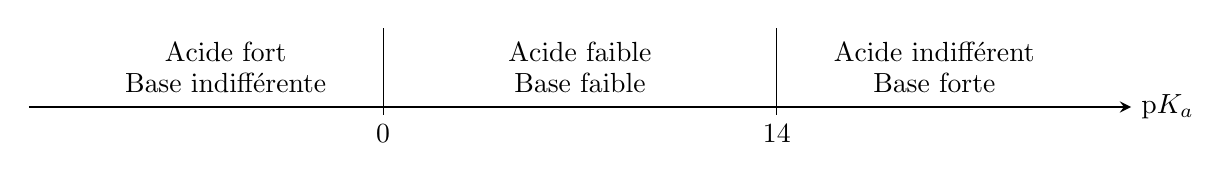
\begin{tikzpicture}[baseline=1em]
        \draw[->, >=stealth, thick] (-7,0)--(7,0) node[right]{p$K_a$};
        \draw[black] (-2.5,1)--(-2.5,-0.1) node[below]{0} ;
        \draw[black] (2.5,1)--(2.5,-0.1) node[below]{14} ;
        \node at (-4.5,.3) {Base indifférente};
        \node at (0,.3) {Base faible};
        \node at (4.5,.3) {Base forte};
        \node at (-4.5,.7) {Acide fort};
        \node at (0,.7) {Acide faible};
        \node at (4.5,.7) {Acide indifférent};
    \end{tikzpicture}\end{center}
    
    \question $\mathrm{AH \equiv CH_3\text{--}CH_2\text{--}COOH}$, c'est un acide faible.
    
    \question Pour un acide faible, $\text{pH} = \dfrac{1}{2}\qty(\text{p}K_a + \text{p}c)$. Plus on dilue l'acide, et plus il est dissocié.
    
    \question ~ \\[-2.5em]
    \begin{center}\begin{tabularx}{10cm}{r|C|C|C}
&
\multicolumn{1}{|c!{\makebox[0pt]{$\leftrightharpoons$}}}{AH}
&
\multicolumn{1}{c!{\makebox[0pt]{+}}}{A$^-$}
&
H$^+$
\\
\hline\hline
Init. & $c$ & 0 & $10^{-\text{p}K_e/2}$ \\
Eq. & $(1-\alpha)c$ & $\alpha c$ & $10^{-\text{p}K_e/2} + \alpha c$
\end{tabularx}\end{center}
    
    \question\hfill $10^{-\text{p}K_a} = \mathrm{\dfrac{[A^-][H^+]}{[AH]}} = \dfrac{\alpha\qty(10^{-\text{p}K_e/2} + \alpha 10^{-\text{p}c})}{1 - \alpha},$ \hfill ~
    $$\text{d'où}\qquad \alpha^2 + \alpha\qty(10^{\text{p}c - \text{p}K_a} + 10^{\text{p}c - \text{p}K_e/2}) - 10^{\text{p}c-\text{p}K_a} = 0. \qquad (\ast)$$
    
    \question On n'a pas pris en compte l'autoprotoloyse de l'eau. Pour la prendre en compte, il faudrait ajouter un second avancement $\beta$ permettant d'établir deux équations à deux inconnues $\alpha, \beta$.
    
    \question Pour cet acide faible, on a p$K_a \ll \text{p}K_e/2$.
    
    \textbf{\sffamily a)} Dans ce cas, l'équation $(\ast)$ se simplifie en $\alpha = 10^{(\text{p}c-\text{p}K_a)/2}$ et $\text{pH} = \dfrac{1}{2}(\text{p}K_a + \text{p}c)$ (domaine acide faible) ;
    
    \textbf{\sffamily b)} Dans ce cas, l'équation $(\ast)$ se simplifie en $\alpha = 1$ et $\text{pH} = \text{p}c$ (domaine acide fort) ;
    
    \textbf{\sffamily c)} Dans ce cas, l'équation $(\ast)$ se simplifie en $\alpha = 1$ et $\text{pH} = 10^{-\text{p}K_e/2} = 7$ (domaine infiniment dilué) ;
    
    Tout cela est cohérent avec la figure.
    
    \question On voit donc que pour le domaine \textbf{\sffamily b)}, notre acide faible a un comportement d'acide fort.
\end{questions}
\end{solution}